\documentclass[12pt]{article}

\usepackage{amsmath}
\usepackage{amssymb}
\usepackage{graphicx}
\usepackage{listings}
\usepackage{xcolor}
\usepackage{geometry}
\usepackage{hyperref}
\usepackage{enumitem}
\usepackage{caption}
\usepackage{booktabs}
\usepackage{array}
\usepackage{tikz}
\usepackage{textcomp}

\graphicspath{{./screenshots/}}
\geometry{margin=1in}
\setlength{\parindent}{0pt}
\setlength{\parskip}{6pt}
\setcounter{secnumdepth}{0}
\tolerance=1000
\emergencystretch=\maxdimen

\lstset{
    basicstyle=\ttfamily\small,
    keywordstyle=\color{blue},
    commentstyle=\color{gray},
    stringstyle=\color{orange},
    numbers=left,
    numberstyle=\tiny,
    breaklines=true,
    columns=fullflexible,
    frame=single,
    backgroundcolor=\color{gray!10}
}

\begin{document}

\begin{center}
    {\LARGE \textbf{RBE 500 -- Homework 5}} \\[6pt]
    {\large Tracy Yang} \\[4pt]
    {\large \today}
\end{center}

%=============================================================
\section{Part 1-A: Velocity Kinematics of ABB IRB1400}

Same DH parameters as HW3 and HW4:

\begin{center}
\renewcommand{\arraystretch}{1.3}
\begin{tabular}{ccccc}
\toprule
Joint $i$ & $\theta_i$ & $d_i$ (mm) & $a_i$ (mm) & $\alpha_i$ \\
\midrule
1 & $q_1$                & 475 & 150 & $+90^\circ$ \\
2 & $q_2 + 90^\circ$     &   0 & 600 & $0^\circ$   \\
3 & $q_3$                &   0 & 120 & $+90^\circ$ \\
4 & $q_4 + 90^\circ$     & 720 &   0 & $+90^\circ$ \\
5 & $q_5$                &   0 &   0 & $-90^\circ$ \\
6 & $q_6$                &  85 &   0 & $0^\circ$   \\
\bottomrule
\end{tabular}
\end{center}

%-------------------------------------------------------------
\subsection{Question 1: $6 \times 6$ Manipulator Jacobian}

Since all six joints are revolute, each column of $J$ is:
\[
J_i =
\begin{bmatrix}
z_{i-1}^0 \times (p_e^0 - p_{i-1}^0) \\[4pt]
z_{i-1}^0
\end{bmatrix}
\]

where $z_{i-1}^0$ is the $z$-axis of frame $i-1$ in the base frame,
$p_e^0$ is the EE position, and $p_{i-1}^0$ is the origin of frame $i-1$.

Column 1 is the simplest since $z_0^0 = [0,\,0,\,1]^T$:
\[
J_{l1} = \begin{bmatrix}0\\0\\1\end{bmatrix} \times
         \begin{bmatrix}p_{ex}\\p_{ey}\\p_{ez}\end{bmatrix}
       = \begin{bmatrix}-p_{ey}\\p_{ex}\\0\end{bmatrix},
\qquad
J_{a1} = \begin{bmatrix}0\\0\\1\end{bmatrix}
\]

The remaining columns follow the same pattern. Applying the trig
identities $\sin(q+90^\circ)=\cos q$ and $\cos(q+90^\circ)=-\sin q$
to simplify the DH joint offsets, the $z$-axes work out to:

\begin{center}
\renewcommand{\arraystretch}{1.4}
\begin{tabular}{cl}
\toprule
Axis & Expression \\
\midrule
$z_0$ & $[0,\;0,\;1]^T$ \\
$z_1$ & $[\sin q_1,\;{-\cos q_1},\;0]^T$ \\
$z_2$ & $[\sin q_1,\;{-\cos q_1},\;0]^T$ \quad ($\alpha_2=0$, so $z_2 \parallel z_1$) \\
$z_3$ & $[c_1 c_{23},\;s_1 c_{23},\;{-s_{23}}]^T$ \quad ($c_{23}=\cos(q_2+q_3)$, $s_{23}=\sin(q_2+q_3)$) \\
$z_4$ & $[{-c_1 c_{23} s_4 - s_1 c_4},\;{-s_1 c_{23} s_4 + c_1 c_4},\;s_{23} s_4]^T$ \\
$z_5$ & $[c_1 c_{23} c_4 s_5 - s_1 s_4 s_5 + c_1 s_{23} c_5,\;\ldots]^T$ \\
\bottomrule
\end{tabular}
\end{center}

The lower half of $J$ is just $J_a = [z_0\mid z_1\mid z_2\mid z_3\mid z_4\mid z_5]$,
and the upper half uses the cross-product formula with these axes and the
EE position from $T_6^0$.

The following MATLAB code builds and evaluates $J$ numerically:

\begin{lstlisting}[language=Matlab, caption={MATLAB: $6\times6$ Jacobian for ABB IRB1400}]
syms q1 q2 q3 q4 q5 q6 real

dh = @(th,d,a,al) ...
    [cos(th) -sin(th)*cos(al)  sin(th)*sin(al) a*cos(th);
     sin(th)  cos(th)*cos(al) -cos(th)*sin(al) a*sin(th);
     0        sin(al)          cos(al)          d;
     0        0                0                1];

d1=475; a1=150; a2=600; a3=120; d4=720; d6=85;

T01 = dh(q1,        d1,a1, pi/2);  T12 = dh(q2+pi/2, 0,a2,    0);
T23 = dh(q3,         0,a3, pi/2);  T34 = dh(q4+pi/2,d4, 0, pi/2);
T45 = dh(q5,         0, 0,-pi/2);  T56 = dh(q6,     d6, 0,    0);

T02=T01*T12; T03=T02*T23; T04=T03*T34; T05=T04*T45; T06=T05*T56;

z0=[0;0;1]; p0=[0;0;0];
z1=T01(1:3,3); p1=T01(1:3,4);
z2=T02(1:3,3); p2=T02(1:3,4);
z3=T03(1:3,3); p3=T03(1:3,4);
z4=T04(1:3,3); p4=T04(1:3,4);
z5=T05(1:3,3); p5=T05(1:3,4);
pe=T06(1:3,4);

J = sym(zeros(6,6));
J(:,1)=[cross(z0,pe-p0);z0];  J(:,2)=[cross(z1,pe-p1);z1];
J(:,3)=[cross(z2,pe-p2);z2];  J(:,4)=[cross(z3,pe-p3);z3];
J(:,5)=[cross(z4,pe-p4);z4];  J(:,6)=[cross(z5,pe-p5);z5];

% Evaluate numerically at HW4 Part 1.3 configuration
q_vals = [11.31, 24.96, -1.57, 0, 0, 0] * pi/180;
J_num = double(subs(J, [q1,q2,q3,q4,q5,q6], q_vals));
disp(round(J_num, 4));
\end{lstlisting}

The symbolic Jacobian entries are too large to print (each element is several lines of nested trig), so the numerical result at the HW4 configuration is shown below in Figure~\ref{fig:jacobian_out}.

\begin{figure}[h]
    \centering
    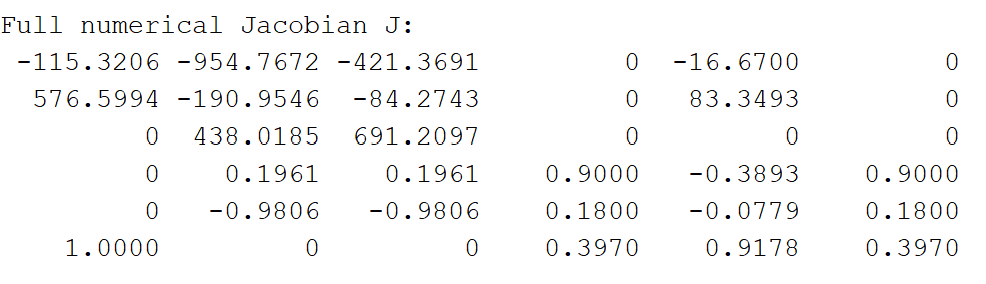
\includegraphics[width=0.82\textwidth]{jacobian_out.png}
    \caption{MATLAB output: $6\times6$ Jacobian evaluated numerically at $\mathbf{q} = [11.31^\circ, 24.96^\circ, -1.57^\circ, 0^\circ, 0^\circ, 0^\circ]$.}
    \label{fig:jacobian_out}
\end{figure}
% Save screenshot of disp(round(J_num,4)) as screenshots/jacobian_out.png

%-------------------------------------------------------------
\subsection{Question 2: Joint Velocities}

Fixing the wrist at zero ($q_4=q_5=q_6=0$) and using the joint
angles from HW4 Part~1.3:
\[
\mathbf{q} = [11.31^\circ,\;24.96^\circ,\;-1.57^\circ,\;0^\circ,\;0^\circ,\;0^\circ]
\]

The full numerical Jacobian at this configuration is shown in Figure~\ref{fig:jacobian_out}.
With the wrist fixed, only joints 1--3 affect the EE linear velocity,
so we pull out the top-left $3\times3$ block and solve:
\[
\dot{\mathbf{x}} = J_l^{(3)}\,\dot{\mathbf{q}}_{1:3}
\quad\Rightarrow\quad
\dot{\mathbf{q}}_{1:3} = \left(J_l^{(3)}\right)^{-1}\dot{\mathbf{x}}
\]

\[
J_l^{(3)} =
\begin{bmatrix}
-115.32 & -954.77 & -421.37 \\
 576.60 & -190.95 &  -84.27 \\
    0   &  438.02 &  691.21
\end{bmatrix}, \qquad
\det\!\left(J_l^{(3)}\right) = 2.851\times10^8 \neq 0
\]

\[
\left(J_l^{(3)}\right)^{-1}
  \begin{bmatrix}5\\5\\10\end{bmatrix}
=
\begin{bmatrix}
\phantom{-}0.0067 \\
-0.0173 \\
\phantom{-}0.0254
\end{bmatrix}
\text{ rad/s}
\quad\Leftrightarrow\quad
\begin{bmatrix}
\phantom{-}0.38 \\
-0.99 \\
\phantom{-}1.46
\end{bmatrix}
\text{ deg/s}
\]

Verification: $J_l^{(3)}\,\dot{\mathbf{q}}_{1:3} = [5.00,\;5.00,\;10.00]^T$\,mm/s\;\checkmark

%-------------------------------------------------------------
\subsection{Question 3: Singular Configurations}

Remove the wrist and set $d_6=0$, $q_4=q_5=q_6=0$, leaving a
3-DOF arm. Per the hint, use only the linear half of $J$, which
becomes the $3\times3$ matrix $J_l$. The arm is singular when
$\det(J_l) = 0$.

\subsubsection*{Shoulder Singularity}

Column 1 of $J_l$ is:
\[
z_0 \times (p_e - p_0) = [0,0,1]^T \times [p_{ex},\,p_{ey},\,p_{ez}]^T
= [-p_{ey},\;p_{ex},\;0]^T
\]

This goes to zero when $p_{ex} = p_{ey} = 0$, i.e.\ the EE is
directly above the base on the $z_0$ axis. At that point joint 1
spinning has no effect on EE position, so $\det(J_l) = 0$.

The horizontal reach is $R(q_2,q_3) = a_1 + a_2\sin(q_2+90^\circ)
+ a_3\cos(q_2+90^\circ+q_3) + d_4\sin(q_2+90^\circ+q_3)$, and
the singularity occurs whenever $R=0$. Solving numerically gives
one example: $q_1=0^\circ$, $q_2\approx-143.47^\circ$, $q_3=0^\circ$,
at which $\det(J_l)=0$ and $\mathrm{rank}(J_l)=2$.

\subsubsection*{Elbow Singularity}

Because this robot has both $a_3=120$\,mm and $d_4=720$\,mm, the
effective elbow link is $L=\sqrt{a_3^2+d_4^2}=729.9$\,mm at
internal angle $\phi=\arctan(d_4/a_3)=80.5^\circ$. The elbow
singularity does not fall at simple angles like $q_3=0^\circ$ or
$180^\circ$ — it happens wherever the arm hits its workspace boundary.

The symbolic determinant (computed in MATLAB) depends only on $q_2$
and $q_3$ (independent of $q_1$ by symmetry). After simplification:
\[
\det(J_l) \propto
600\sin(q_2+q_3) - 120\cos(q_2+q_3) - 600\sin q_2\sin(q_2+q_3)
+ 120\sin q_2\cos(q_2+q_3)
\]
which can be written as $L\sin(q_2+q_3-q_2) \cdot (\ldots)$, showing
the zeros occur at workspace boundary configurations. Setting this to
zero and scanning $q_3\in[-180^\circ,180^\circ]$ at $q_1=30^\circ$,
$q_2=45^\circ$ finds four zeros:
\[
q_3 \in \{-122.39^\circ,\;-99.46^\circ,\;13.47^\circ,\;80.54^\circ\}
\]

At each, rank drops to 2. Note that $q_3=80.54^\circ=\phi$, which
is the arm-straight condition in this DH convention.

\textbf{Summary:}
\[
\begin{cases}
\textbf{Shoulder:} & R(q_2,q_3) = 0
  \quad\text{(EE on } z_0\text{ axis, e.g.\ } q_2\approx-143.5^\circ) \\[4pt]
\textbf{Elbow:}    & q_3 \in \{-122.4^\circ,\,-99.5^\circ,\,13.5^\circ,\,80.5^\circ\}
\end{cases}
\]

For the full 6-DOF robot there is also a wrist singularity at
$q_5=0^\circ$, where joints 4 and 6 become co-axial.

%=============================================================
\newpage
\section{Part 1-B: Textbook Problems (Spong, 2nd Edition)}

%-------------------------------------------------------------
\subsection{Problem 4-15: Cylindrical Manipulator (Figure 3.7)}

\begin{figure}[h]
    \centering
    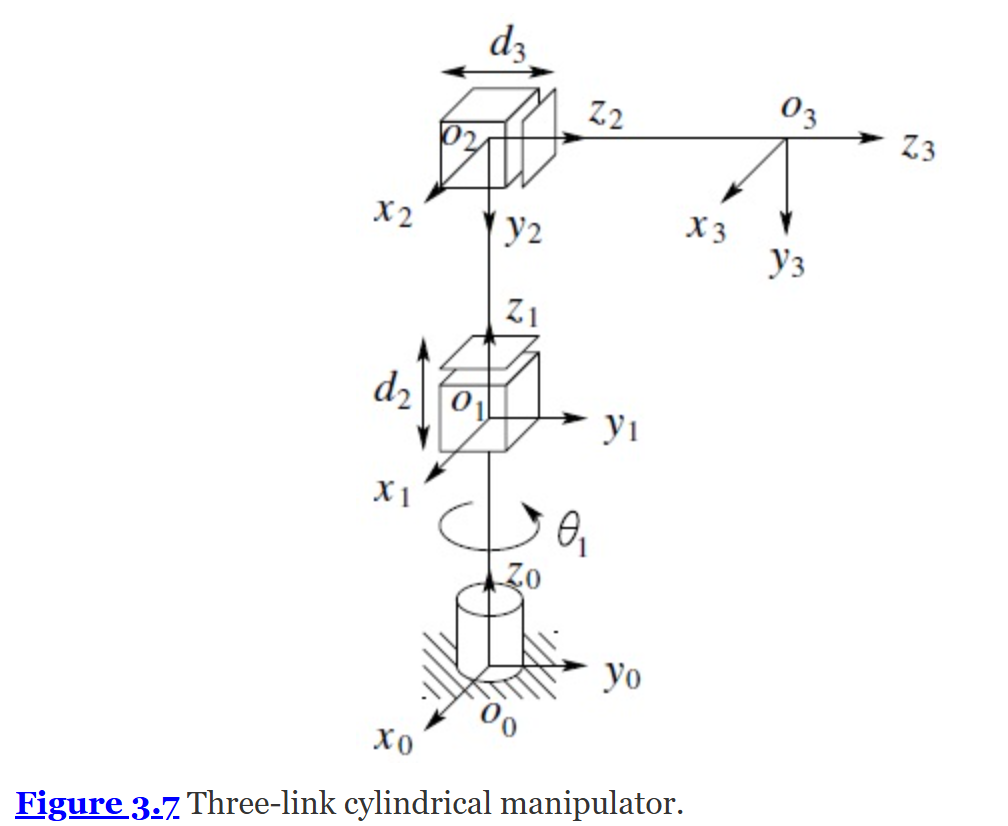
\includegraphics[width=0.45\textwidth]{fig3_7.png}
    \caption{Three-link cylindrical manipulator (Spong Figure~3.7). Joint sequence: RPP.}
    \label{fig:fig37}
\end{figure}

Joint sequence is RPP: joint 1 revolute ($\theta_1$), joints 2 and 3
prismatic ($d_2$, $d_3$).

\textbf{DH parameters:}
\begin{center}
\renewcommand{\arraystretch}{1.3}
\begin{tabular}{ccccc}
\toprule
Joint $i$ & $\theta_i$ & $d_i$ & $a_i$ & $\alpha_i$ \\
\midrule
1 & $q_1$ & $0$   & $0$ & $-90^\circ$ \\
2 & $0$   & $d_2$ & $0$ & $0^\circ$   \\
3 & $0$   & $d_3$ & $0$ & $0^\circ$   \\
\bottomrule
\end{tabular}
\end{center}

\textbf{Axes and origins:}
\begin{align*}
z_0 &= [0,0,1]^T,      & p_0 &= [0,0,0]^T \\
z_1 &= [0,0,1]^T,      & p_1 &= [0,0,0]^T \\
z_2 &= [-s_1,c_1,0]^T, & p_2 &= [0,0,d_2]^T
\end{align*}

EE position: $p_e = [-s_1 d_3,\; c_1 d_3,\; d_2]^T$.

\textbf{Jacobian columns:}

Joint 1 (revolute):
\[
J_{l1} = z_0 \times (p_e - p_0)
= \begin{bmatrix}0\\0\\1\end{bmatrix}\times\begin{bmatrix}-s_1 d_3\\c_1 d_3\\d_2\end{bmatrix}
= \begin{bmatrix}-c_1 d_3\\-s_1 d_3\\0\end{bmatrix},
\qquad
J_{a1} = \begin{bmatrix}0\\0\\1\end{bmatrix}
\]

Joints 2 and 3 (prismatic, so $J_{li}=z_{i-1}$ and $J_{ai}=\mathbf{0}$):
\[
J_{l2} = z_1 = \begin{bmatrix}0\\0\\1\end{bmatrix}, \qquad
J_{l3} = z_2 = \begin{bmatrix}-s_1\\c_1\\0\end{bmatrix}
\]

\textbf{Full $6\times3$ Jacobian:}
\[
J =
\begin{bmatrix}
-c_1 d_3 & 0 & -s_1 \\
-s_1 d_3 & 0 &  c_1 \\
0         & 1 &  0   \\
0         & 0 &  0   \\
0         & 0 &  0   \\
1         & 0 &  0
\end{bmatrix}
\]

\textbf{Singularities:} Expanding $\det(J_l)$ along the third row:
\[
\det(J_l) = 1\cdot\det\begin{bmatrix}-c_1 d_3 & -s_1\\-s_1 d_3 & c_1\end{bmatrix}
= -d_3(c_1^2 + s_1^2) = -d_3
\]
\[
\boxed{\det(J_l) = 0 \;\Longleftrightarrow\; d_3 = 0}
\]

The only singularity is when $d_3=0$, meaning the EE is sitting on
the $z_0$ rotation axis and joint 1 spinning does nothing.

%-------------------------------------------------------------
\subsection{Problem 4-16: Cartesian Manipulator (Figure 3.17)}

\begin{figure}[h]
    \centering
    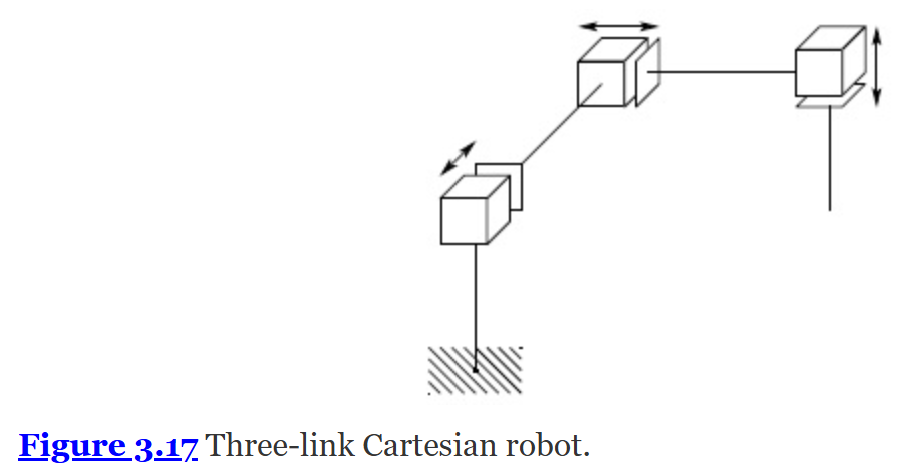
\includegraphics[width=0.5\textwidth]{fig3_17.png}
    \caption{Three-link Cartesian manipulator (Spong Figure~3.17). Joint sequence: PPP.}
    \label{fig:fig317}
\end{figure}

All three joints are prismatic, translating along fixed orthogonal axes:
$z_0=[0,0,1]^T$, $z_1=[0,1,0]^T$, $z_2=[1,0,0]^T$.

For prismatic joints $J_{li}=z_{i-1}$ and $J_{ai}=\mathbf{0}$, so:
\[
J =
\begin{bmatrix}
0 & 0 & 1 \\
0 & 1 & 0 \\
1 & 0 & 0 \\
0 & 0 & 0 \\
0 & 0 & 0 \\
0 & 0 & 0
\end{bmatrix}
\]

$\det(J_l) = -1 \neq 0$ for all joint values, so this robot has
\textbf{no singularities}. The three axes are always orthogonal and
independent no matter where the joints move.

%-------------------------------------------------------------
\subsection{Problem 4-17: Stanford Manipulator (Completing Example 4.7)}

\begin{figure}[h]
    \centering
    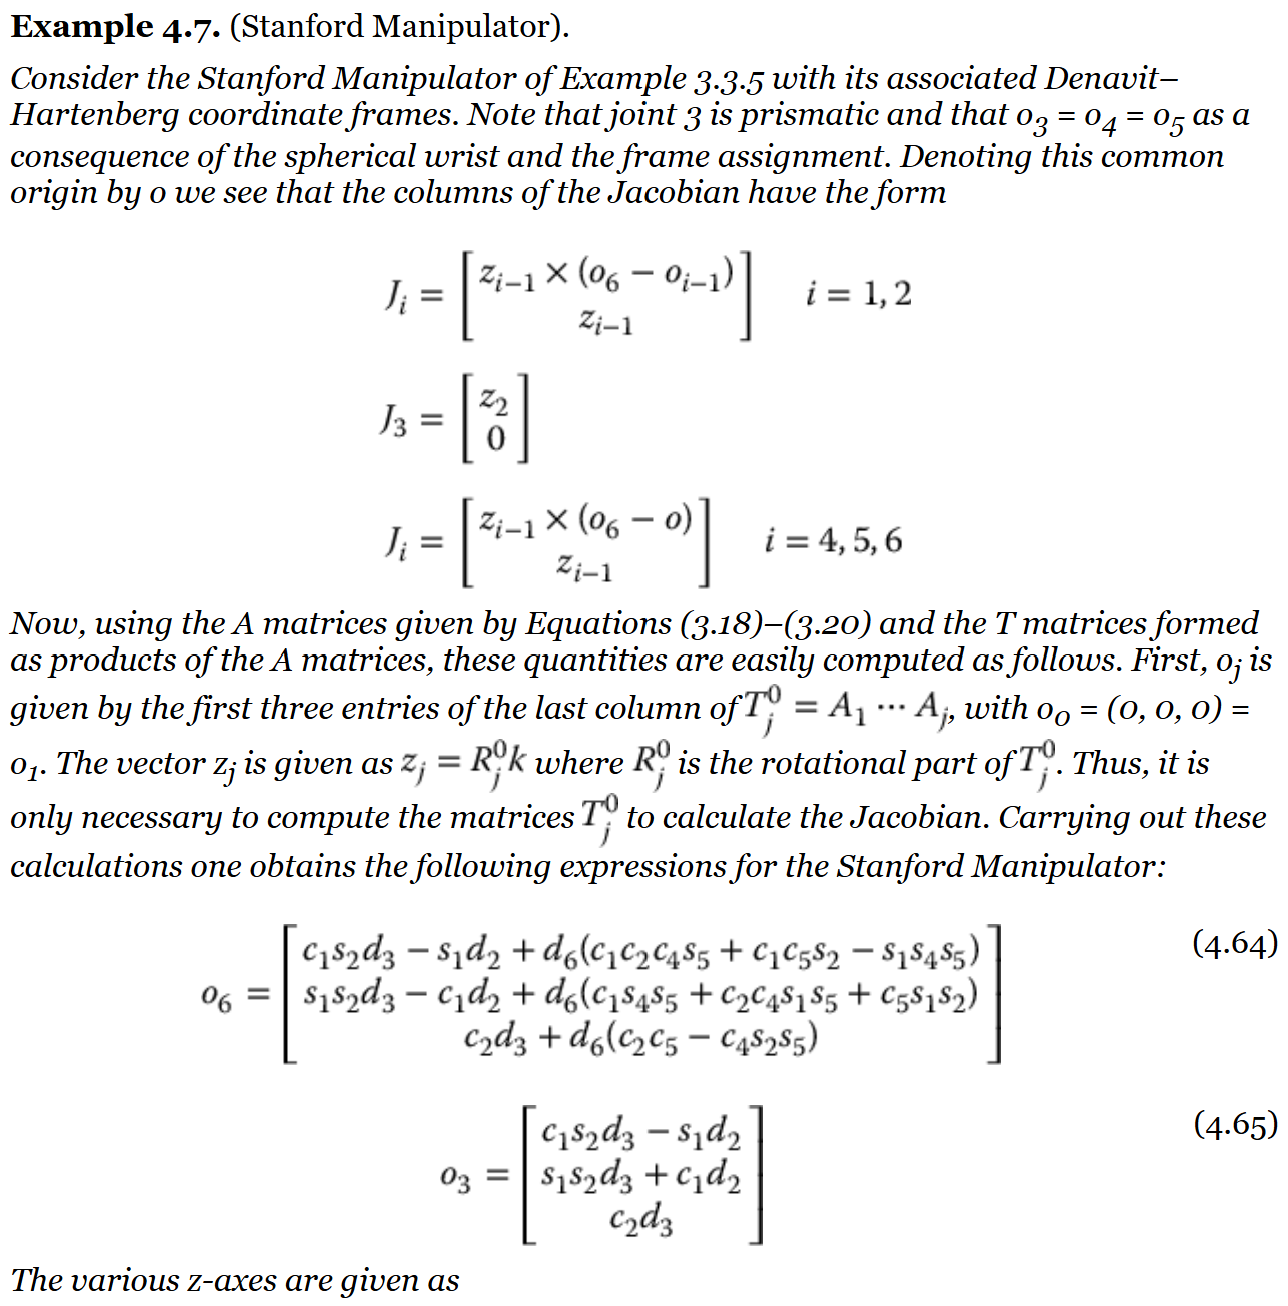
\includegraphics[width=0.82\textwidth]{ex4_7_1.png}\\[6pt]
    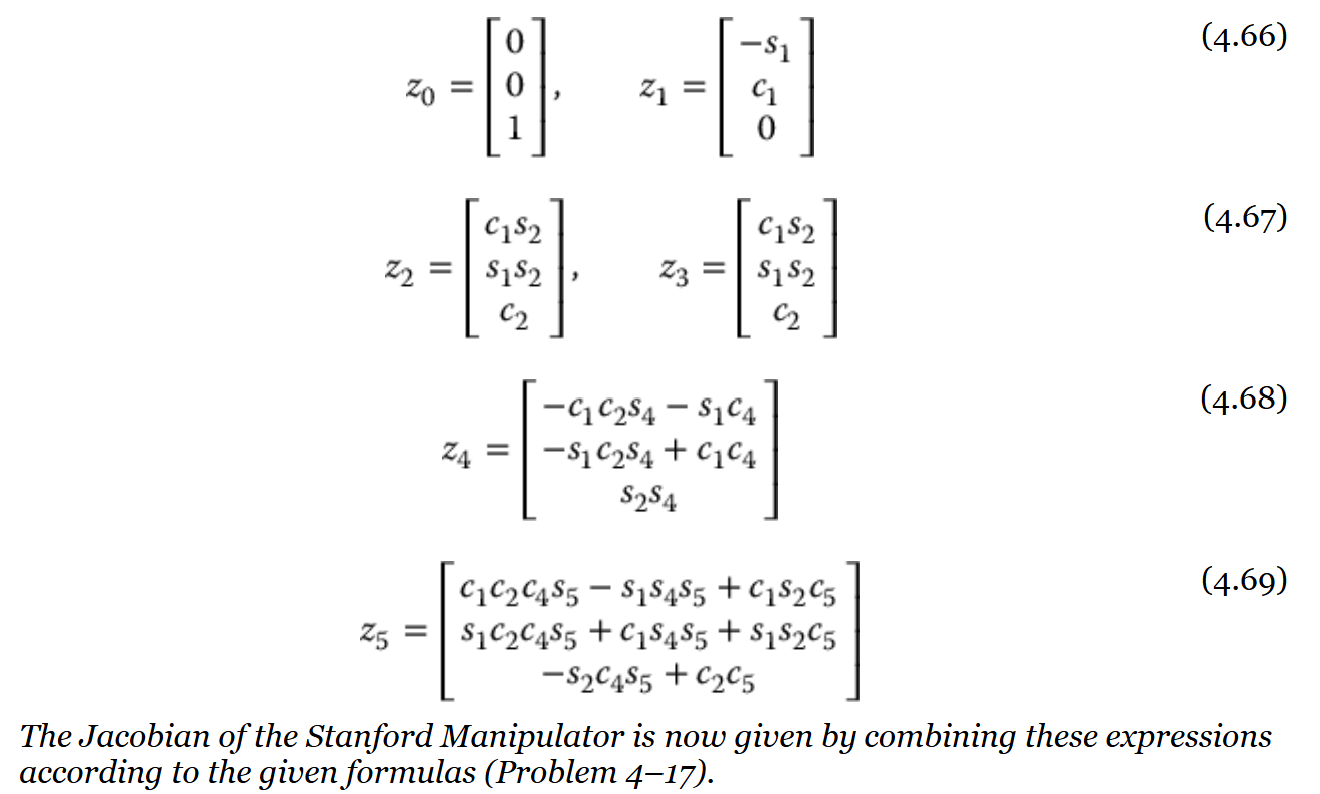
\includegraphics[width=0.82\textwidth]{ex4_7_2.png}
    \caption{Example 4.7: column templates, EE position $o_6$, wrist center $o_3$ (top),
             and $z$-axis expressions $z_0$--$z_5$ from Eq.\ 4.66--4.69 (bottom).}
    \label{fig:ex47}
\end{figure}

The example gives us $o_6$, $o_3$, and all the $z$-axes. The spherical
wrist means $o_3=o_4=o_5\triangleq o$, so the vector from the wrist
center to the EE is simply $o_6-o=d_6\,z_5$.

The column formulas from the example are:
\[
J_i = \begin{bmatrix}z_{i-1}\times(o_6-o_{i-1})\\z_{i-1}\end{bmatrix}\ (i=1,2),
\quad
J_3 = \begin{bmatrix}z_2\\\mathbf{0}\end{bmatrix},
\quad
J_i = \begin{bmatrix}z_{i-1}\times(o_6-o)\\z_{i-1}\end{bmatrix}\ (i=4,5,6)
\]

Filling these in:

\textit{Column 3} (prismatic, $z_2=[c_1 s_2,\,s_1 s_2,\,c_2]^T$):
\[
J_3 = \begin{bmatrix}c_1 s_2 \\ s_1 s_2 \\ c_2 \\ 0 \\ 0 \\ 0\end{bmatrix}
\]

\textit{Columns 4--6} (wrist, all share origin $o$, so $o_6-o=d_6 z_5$):
\[
J_{l4} = z_3\times d_6 z_5,\quad
J_{l5} = z_4\times d_6 z_5,\quad
J_{l6} = z_5\times d_6 z_5 = \mathbf{0}
\]
\[
J_{a4} = z_3,\quad J_{a5} = z_4,\quad J_{a6} = z_5
\]

$J_{l6}=\mathbf{0}$ because joint 6's axis passes through the EE,
so spinning it produces no linear velocity.

\textbf{Complete $6\times6$ Jacobian:}
\[
J = \begin{bmatrix}
z_0\times(o_6-o_0) & z_1\times(o_6-o_1) & z_2
  & z_3\times d_6 z_5 & z_4\times d_6 z_5 & \mathbf{0} \\[4pt]
z_0 & z_1 & \mathbf{0} & z_3 & z_4 & z_5
\end{bmatrix}
\]

Plugging in the expressions from Eq.~(4.64)--(4.69) finishes the derivation.

\end{document}